\subsection{Proxy Re-Encryption}

\subsubsection{Introduction to Proxy Re-Encryption}

\blockquote{In a proxy re-encryption scheme a semi-trusted proxy converts a ciphertext for Alice into a ciphertext for Bob without seeing the underlying plaintext}~\autocite{greenateniese:2006:article}

Fundamentally, proxy re-encryption is the process of taking a message $M_a$, encrypted by a party $P_a$, and re-encrypting it to be passed to party $P_b$. The message is then in the form of $M_b$, such that it is only readable by party $P_b$. Through the re-encryption process, the message is never actually decrypted, such that the data is never revealed to any non-trusted parties (including the proxy itself). This process relies on the functional relationship between the two ciphertexts, with the characteristics of the proxy re-encryption processed determined by the topology of this function.

\begin{figure}[H]
  \centering
  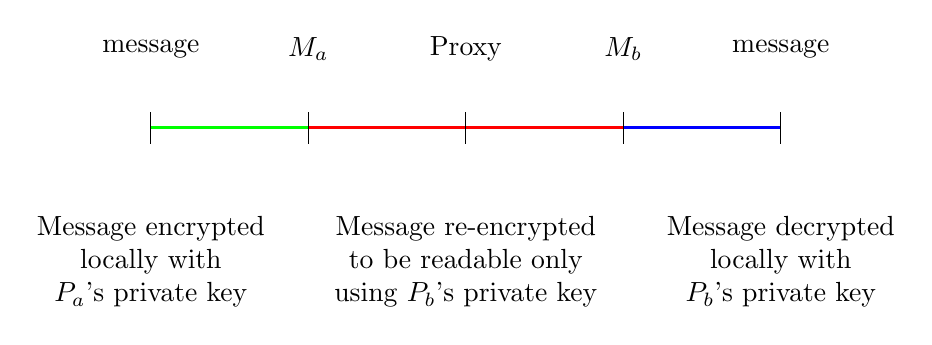
\begin{tikzpicture}

  \node at (0, 1)   {message} ;
  \node at (2, 1)   {$M_a$}   ;
  \node at (4, 1)   {Proxy}   ;
  \node at (6, 1)   {$M_b$}   ;
  \node at (8, 1)   {message} ;

  \draw [very thick, green] (0,0)   -- (2,0)   ;
  \draw [very thick, red]   (2,0)   -- (6,0)   ;
  \draw [very thick, blue]  (6,0)   -- (8,0)   ;
  \draw                     (0,-.2) -- (0, .2) ;
  \draw                     (2,-.2) -- (2, .2) ;
  \draw                     (4,-.2) -- (4, .2) ;
  \draw                     (6,-.2) -- (6, .2) ;
  \draw                     (8,-.2) -- (8, .2) ;

  \node[align=center, below] at (0, -1)%
    {Message encrypted\\locally with\\$P_a$'s private key};
  \node[align=center, below] at (4, -1)%
    {Message re-encrypted\\to be readable only\\using $P_b$'s private key};
  \node[align=center, below] at (8, -1)%
    {Message decrypted\\locally with\\$P_b$'s private key};

  \end{tikzpicture}
  \caption{
    Journey of a message using a proxy re-encryption scheme.
  }
\end{figure}


In figure \ref{fig:pre_example}, whether data is handled or manipulated by a fully trusted entity or not is indicated using green/blue and red lines respectively.

The encrypted message $M_a$ is passed to the semi-trusted proxy along with the re-encryption key (expressed as $f(E_a, e_b)$\footnote{$E_x$ represents the private key of a party $x$, $e_x$ represents the public key of a party $x$,})

% Delegation – allows a message recipient (keyholder) to generate a re-encryption key based on his secret key and the key of the delegated user. This re-encryption key is used by the proxy as input to the re-encryption function, which is executed by the proxy to translate ciphertexts to the delegated user's key. Asymmetric proxy re-encryption schemes come in bi-directional and uni-directional varieties.

% - In a bi-directional scheme, the re-encryption scheme is reversible—that is, the re-encryption key can be used to translate messages from Bob to Charlie, as well as from Charlie to Bob. This can have various security consequences, depending on the application. One notable characteristic of bi-directional schemes is that both the delegator and delegated party (e.g., Charlie and Bob) must combine their secret keys to produce the re-encryption key.
% - A uni-directional scheme is effectively one-way; messages can be re-encrypted from Bob to Charlie, but not the reverse. Uni-directional schemes can be constructed such that the delegated party need not reveal its secret key. For example, Bob could delegate to Charlie by combining his secret key with Charlie's public key.

% Transitivity – Transitive proxy re-encryption schemes allow for a ciphertext to be re-encrypted an unlimited number of times. For example, a ciphertext might be re-encrypted from Bob to Charlie, and then again from Charlie to David and so on. Non-transitive schemes allow for only one (or a limited number) of re-encryptions on a given ciphertext. Currently, there is no known uni-directional, transitive proxy re-encryption scheme. It is an open problem as to whether such constructions are possible.

\subsubsection{Applying Proxy Re-Encryption}



\subsubsection{ZeroDB}
